\textbf{defaultdict} python中的defaultdict,也是一种dict。与传统的dict不同,当传统的dict的key不存在时会Error,但defaultdict不会,而是返回一个默认值。该默认值由创建defaultdict时传入的参数有关:$dd = defaultdict(default_factory)$。

当default\_factory是list时,默认值是[],defaultdict其他常见取值还有:str, set, int, dict。但不可以是defaultdict。

\textbf{glob} python中的一个内置模块,用于查找符合特定规则的文件路劲。如:
\begin{python}
	import glob
	pattern = "./myfloder/prefix-*.txt"
	li = glob.glob(pattern) # 此时li中就包含了所有符合pattern这个模式的文件名
\end{python}


\textbf{np.argsort} 对数组的元素进行排序(默认是从小到大),生成一个新的数组,数组元素是排序后的数组所对应的下标。
\begin{python}
	import numpy as np
	x = np.array([2,1,3,5,4])
	y = np.argsort(x) # y = [1, 0, 2, 4, 3]
	# 从大到小排序
	y = np.argsort(-x) # y = [3, 4, 2, 0, 1]
\end{python}
该方法还有更复杂的使用方法,可以根据参数进行调节,$argsort(a, axis=-1, kind=None, order=None)$。

\textbf{numpy设置随机数种子} $np.random.seed(seed)$。

\textbf{python format用法}
\textbf{对齐}"$\{:\}$" 通常将对齐符号放在$:$后。\^ 、| < | >分别是居中、左对齐、右对齐,在填充符号后面可带宽度,在$:$后可带填充字符,默认为空格。

\textbf{数字输出格式}主要包括小数位数(如.2f)、百分号输出(如.2\%)、指数形式输出(如.2e)、带正负符号的输出(如+.2f)、按不同进制的输出(b、d、o、x分别是二进制、十进制、八进制、十六进制,在b|o|x前加\#可以输出进制符号,x的大小写会影响进制符号的大小写。
\begin{python}
	"{:^8}".format("居中")	# 居中显示,宽度为8,默认用空格填充
	"{:*<8}".format("左对齐")	# 左对齐显示,宽度为8,用*填充
	"{:*>8}".format("右对齐")	# 右对齐显示,宽度为8,默认用空格填充
	"{:.2f}".format(123)
	"{:.2%}".format(123)
	"{:^8.2f}".format(123)		# 八位的显示宽度,保留2位小数
	"{:b}".format(11)
	"{:d}".format(11)
	"{:o}".format(11)
	"{:x}".format(11)
	"{:#x}".format(11)
	"{:#X}".format(11)
\end{python}

\textbf{numpy nan的处理}numpy中可以使用np.isnan()来判断数组中的元素是否为NAN,返回的结果与数组形状相同,元素为True/False,该位置的元素为NAN是则为True,否则为False。可以使用 np.nan\_to\_num(x, copy=True, nan=0, posinf= 1.7976931348623157e+308, neginf=-1.7976931348623157e+308) 来进行转换。该函数可以将NAN(包括无穷小、无穷大)转换为数字,可以指定转换后的数字。参数:x是待转换的数据,可以是数组或单个数字;copy表示是否进行原地转换,相当于pandas中的in\_place参数,但取值与in\_place相反;nan表示取代NAN的数字;posinf、neginf表示用什么取代正/负无穷。

\tbc{red}{找到数组中nan指的位置}:np.argwhere(np.isnan(a))。解释:通过np.isnan标记数组中nan值的位置为True,np.argwhere会返回那些True的下标。


\textbf{matplotlib中的marker}如图\ref{fig:matplotlib-markers}所示,更多内容可参见:\href{https://matplotlib.org/api/_as_gen/matplotlib.pyplot.plot.html#matplotlib.pyplot.plot}{Matplotlib}
\begin{figure}[h]
	\centering
	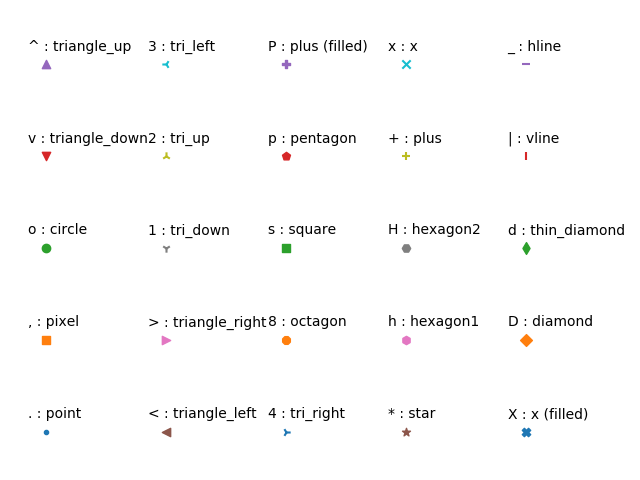
\includegraphics[width=.65\textwidth]{pics/markers.png}
	\caption{Matplotlib中的markers}
	\label{fig:matplotlib-markers}
\end{figure}

\textbf{matplotlib Animation}
Animation可用于制作动画。初始化函数:
\begin{python}
	def __init__(self, fig, func, frames=None, init_func=None, fargs=None,
	save_count=None, *, cache_frame_data=True, **kwargs)
	"""
	fig: 绘制动画的地方
	func: 完成动画动作的回调函数。定义应为:def func(frame, *fargs) -> iterable_of_artists
	frames: 可以认为是每一个动画帧的索引,通常为iterable对象,frames中的每个值会逐个作为func的第一个参数传入
	init_func: 在绘制第一帧之前调用的函数,定义应为:def init_func() -> iterable_of_artists
	fargs: 用于func的额外的参数
	repeat_delay: 帧之间的延迟,单位为毫秒
	repeat: 是否重复播放动画
	blit: 布尔值故, 默认为False。用于优化绘图,注意这个参数有点坑,当其为True时,会根据artists的zorder来绘图,当对象没有zorder(如bar)时则会报错
	"""
\end{python}
在使用matplotlib制作动画的过程中,很重要的是要知道要让什么对象发生变化、发生什么变化 --- 知道了这二者之后就可以在每一帧的更新函数中完成对应的动作了。

\tbc{red}{注意}:blit参数的使用,当启用了blit时,且要对bar改变时,则会报错:\textit{AttributeError: 'BarContainer' object has no attribute 'get\_zorder'},把blit设为False即可。


\textbf{matplotlib 调整子图间距}
\begin{itemize}
	\item plt.tight\_layout()
	\item plt.subplot\_adjust(left=None, bottom=None, right=None, top=None, wspace=None, hspace=None)
\end{itemize}

\textbf{matplotlib 显示中文}
\begin{python}
	plt.rcParams['font.sans-serif'] = ['SimHei'] # 步骤一(替换sans-serif字体)  
	plt.rcParams['axes.unicode_minus'] = False  # 步骤二(解决坐标轴负数的负号显示问题)
\end{python}






